\begin{scanpage}{0061}{44}
\begin{minipage}[t]{.45\linewidth}\vspace{0pt}\centering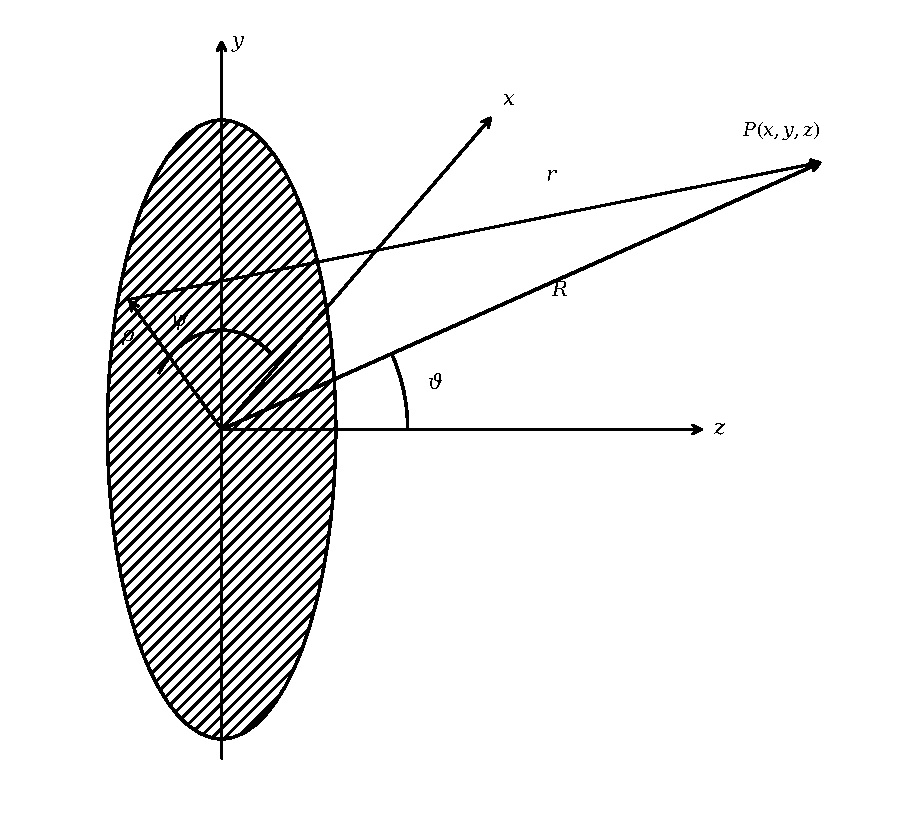
\includegraphics[width=.8\linewidth]{images/recreated/a-0061-fig17.pdf}\par Figure 17. Diffraction by a disk of a plane wave propagated along the $z$ axis.\end{minipage}\hfill\begin{minipage}[t]{.51\linewidth}\vspace{0pt}
\[\left.\begin{aligned}E_y&=-H_x=-H_{0x}e^{ikz},\\E_x&=H_y=0.\end{aligned}\right\}\tag{7.01}\]
The uniform part of the current excited on the disk by wave (7.01) is determined by Equation (3.01) and has the components
\[j_y^0=-\frac c{2\pi}H_{0x},\quad j_x^0=j_z^0=0.\tag{7.02}\]
Let us find the field created by this current.
\end{minipage}
Since the diffraction field in the far zone $(R\gg ka^2)$ is of interest to us, the vector potential
\[\mathbf A(x,y,z)=\frac1c\int_0^a\rho\,d\rho\int_0^{2\pi}\mathbf j(\rho,\psi)\frac{e^{ikr}}r\,d\psi\tag{7.03}\]
may be simplified by using the relationship
\[r=\sqrt{R^2+\rho^2-2\rho R\cos\Omega}\approx R-\rho\cos\Omega,\tag{7.04}\]
where $\Omega$ is the angle between $\rho$ and $R$, and
\[\cos\Omega=\sin\theta\cos(\psi-\phi).\tag{7.05}\]
As a result, we obtain the simpler equation
\[\mathbf A(x,y,z)=\frac1c\frac{e^{ikR}}R\int_0^a\rho\,d\rho\int_0^{2\pi}\mathbf j(\rho,\psi)e^{-ik\rho\cos\Omega}\,d\psi.\tag{7.06}\]
Continuing by using the equations
\[\mathbf H=\operatorname{rot}\mathbf A,\quad\operatorname{rot}\mathbf H=-ik\mathbf E,\tag{7.07}\]
it is easy to show that in the spherical coordinate system the fringing field components with $R\gg ka^2$ equal
\end{scanpage}
